\section{New Method}
In the coming many-core era, due to the tight power budget, power efficiency is cricital for
many-core processor design. In the previous work by Dong Hyuk Woo, evaluation of energy
efficiency on the basis of performance and power (PPW) models is developed, which shows the
tendency of PPW with number of cores. We implement the dark silicon and thermal model into
evaluation of PPW to gain a better understanding of PPW in the dark silicon era.
Different from previous work, the performance of the many-core processor is expressed with
the summary of operating frequency of all cores:
\begin{equation}\label{perf}
Perf = \sum_{i=1}^n f_{i}
\end{equation}

However, the $Perf$ is not able to take into account of fraction of computation that can be
parallelized, it should be replaced in further versions.
The average power consumption of the many-core processor is as follows:
\begin{equation}\label{average_power}
W = \frac{P_{1} \times (1-f)+P_{n} \times f/n}{(1-f)+f/n}
\end{equation}

$P_{1}$ is the power consumption during the sequential computation phase, $P_{n}$ is the power consumption during the parallel computation phase. 

$Perf/W$ of a many-core processor is expressed as
\begin{equation}\label{perf/w}
\frac{Perf}{W} = \sum_{i=1}^n f_{i} \times \frac{(1-f)+f/n}{P_{1} \times (1-f)+P_{n} \times f/n}
\end{equation}

\subsection{Power consumption during parallel phase}
$P_{n}$ is made up of the power consumption of n active cores. Please note that in dark silicon
era, $P_{n} = nk$ is not the correct expression. Due to thermal constraint, Dynamic Voltage and
Frequency Scaling(DVFS) is necessary for Thermal Design Power(TDP) consideration. As a result,
the performance of each of the core may degrade with the increase of the number of active cores.
From xx, we have
\begin{equation}\label{gt=bp}
(G - B_{c}A_{s})T(t) + C\frac{dT(t)}{dt}= B_{c}(P_{d}(t) + P_{0})
\end{equation}

By applying thermal model, the effect of temperature on cores can be introduced. 
Through ergodic method, the distribution of light core with the maximum PPW
for number of light core from 1 to n can be specified.


\subsection{Power consumption during sequential phase}

In (2) and (3), $P_{1}$ is consisted of the power consumption of n-1 idle cores and 1 active 
core. The expression of $P_{1} = 1+(n-1)k$ is not implemented, for the power consumption of 
idle cores and active core is not consistant, due to the influence of the temperature.

By appending idle core model into the above mentioned thermal model, the distribution of idle
core and active core with the maximum PPW for number of light core from 1 to n can be specified.

\begin{figure}
\centering
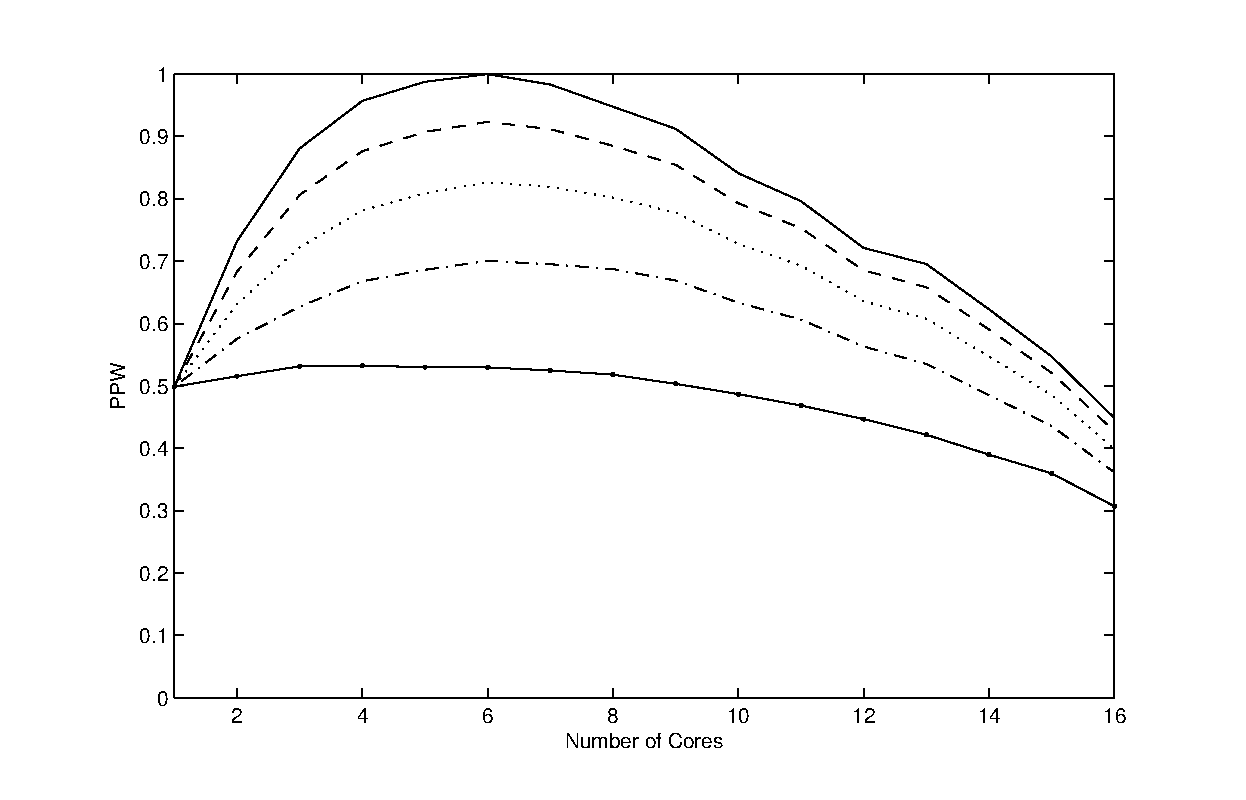
\includegraphics[width=1\columnwidth]{fig/ppw_alpha_ratio.eps}
\caption{The relation between PPW and the number of cores.
}
\label{fig:ppw_alpha_ratio}
\end{figure}